\section{Exp2: Robot reaching}

To investigate whether the previous simulated experiment would generalize to
real robotic arms, robots were set up to do a reaching task, where a central
server maintained a replay buffer, parameters, and executed training.

\subsection{Algorithms and Equipment}

The same setup as in the previous experiment was used with the distributed
version of NAF. The policy was trained on a separate server equipped with a
GPU. Three low-cost robotic arms with three degrees of freedom were used where
different poses were achieved by setting angles of the three servos. A
controller and kinematics were implemented and derived in order to measure and
command poses of the end-effector in cartesian space. For every arm, there was
one dedicated computer, local workers, that evaluated the latest policy given
the arm pose and sent the transitions to the server. The robot with the
coordinate frame is shown in figure \ref{fig:uarm_coordinate_frame} a) and the
entire setup (excluding server) is shown in \ref{fig:uarm_coordinate_frame} b).

\begin{figure}[ht]
    \centering
    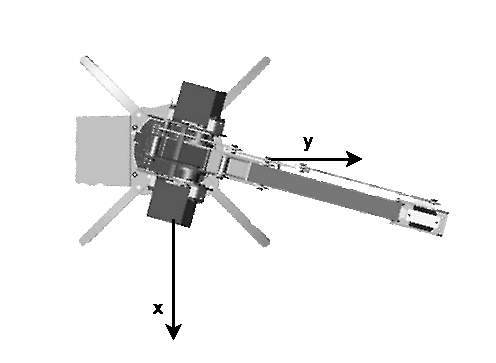
\includegraphics[width=0.39 \textwidth]{res/uarm_coordinates.pdf}
    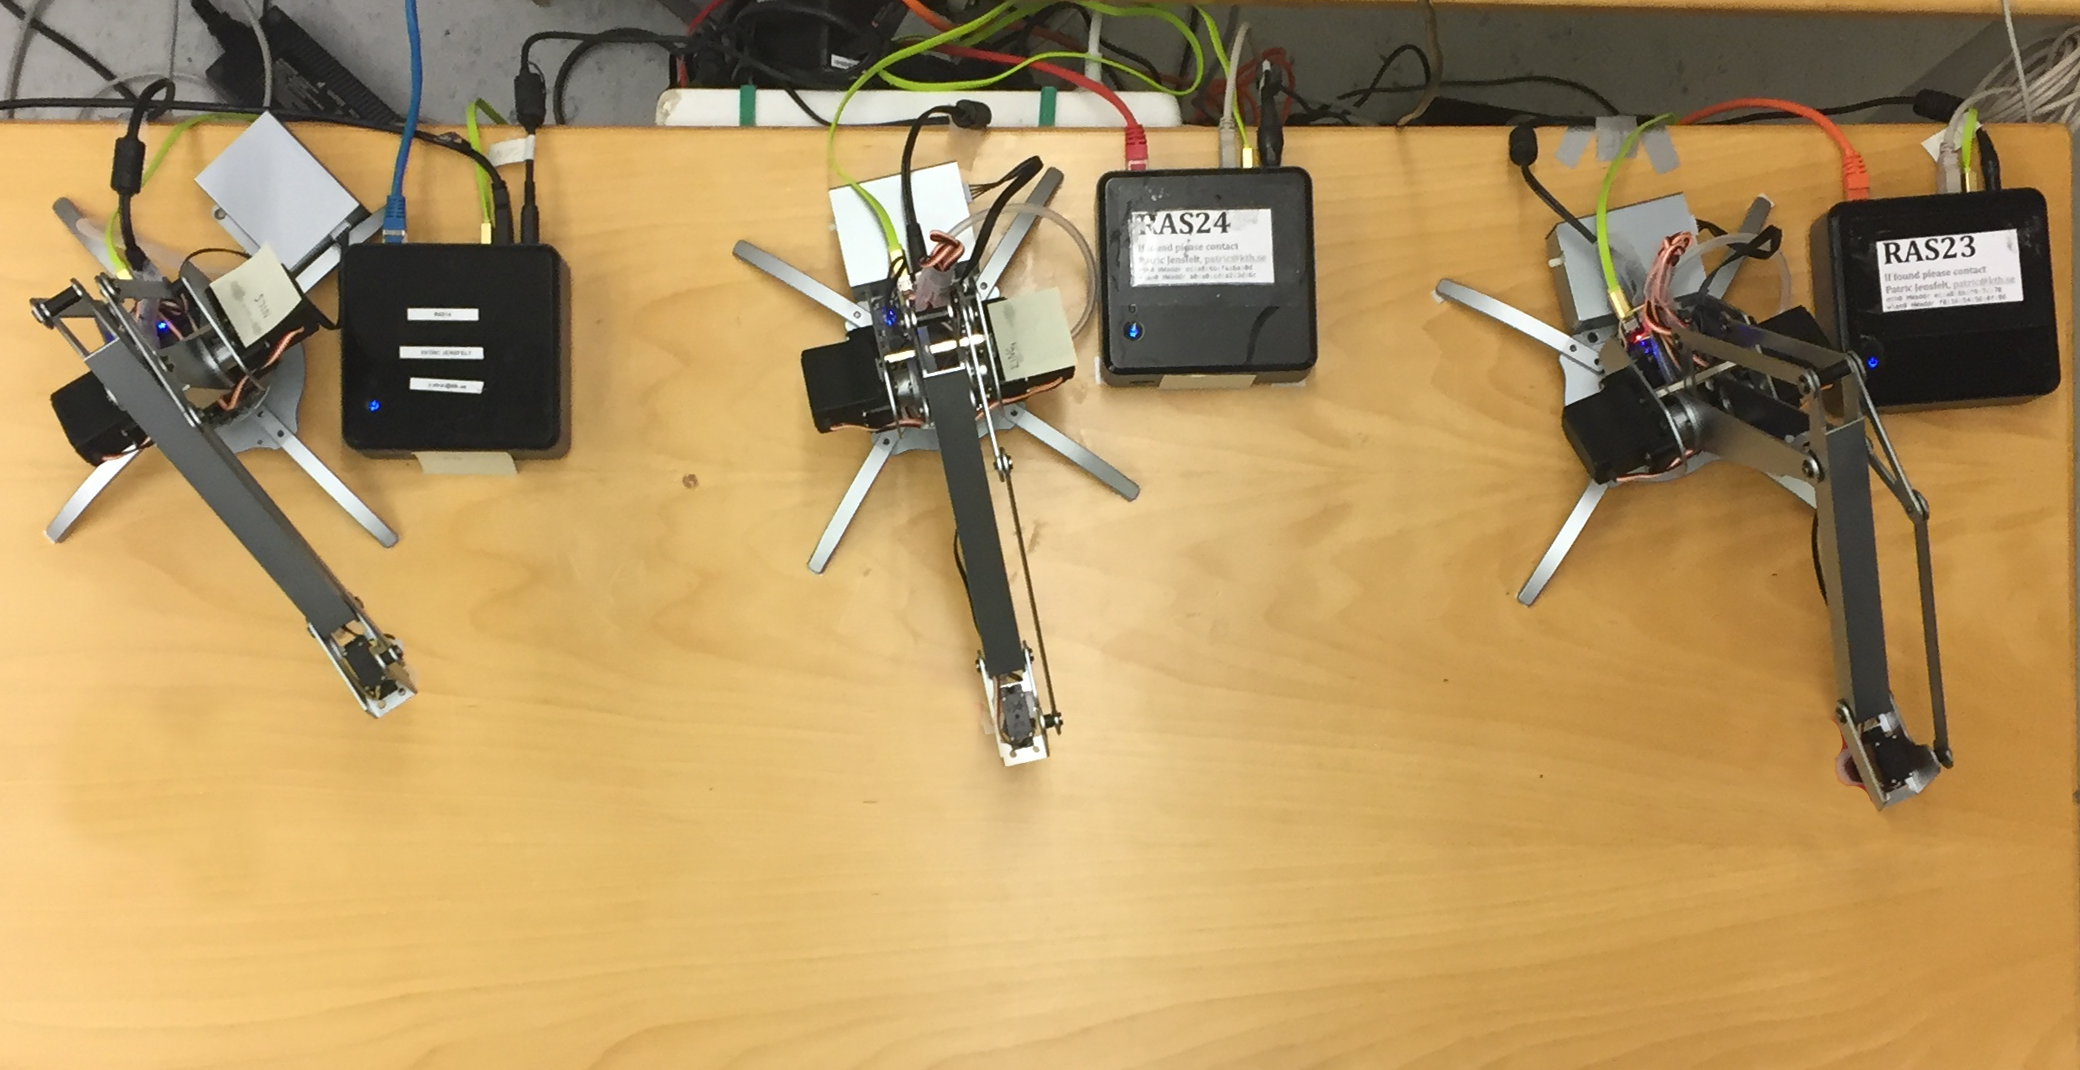
\includegraphics[width=0.59 \textwidth]{res/uarm_moving_setup.png}

    \caption{a) Coordinate frame used. b) The setup of the robot arms along
    with their dedicated computers.}

    \label{fig:uarm_coordinate_frame}
    
\end{figure}

In order to facilitate communication of recorded state transitions and fetching
updated parameters, a server was implemented enabling PUT and GET requests from
the local workers.

\subsection{Data gathering}

Before and after each action was sent to the robot arm, poses of the arm were
measured. This process could only be done at approx. $2-4$ Hz, not including
arm re-positioning, making re-runs from scratch time consuming. Therefore, data
gathering was first run on the three robots for $4$ hours without policy
updates, resulting in approximately $80k$ state transitions. The actions were
randomly drawn from $\mathcal{N}(\mathbf{0}, 0.005^2 \mathbf{I})$, and when the
robot arm reached outside the workspace, or reached within $1$ cm of the
target, the end-effector was replaced at a new random starting position. The
commands were 2-dimensional vectors representing the relative movement in $x$
and $y$ direction respectively. The $z$-coordinate was kept fixed during the
experiment. When training of the parameters was started on the server, the
robots kept collecting and pushing data to the server, and synchronized
parameters before each reset of the end-effector position. During this phase,
noise was added to the policy during every 3 out of 4 runs, while every 1 out 4
runs the policy was evaluated without noise in order to track progress.

\subsection{Results}

The performance of the policy was evaluated by measuring the average distance
to the target position on the last state before every reset. The progress of
this metric is shown in figure \ref{fig:uarm_moving_goal_progress}, here shown
with a running mean of width $128$. The trained policy and value function are
shown in figure \ref{fig:uarm_moving_goal_policy}.

\begin{figure}[h!]
    \centering
    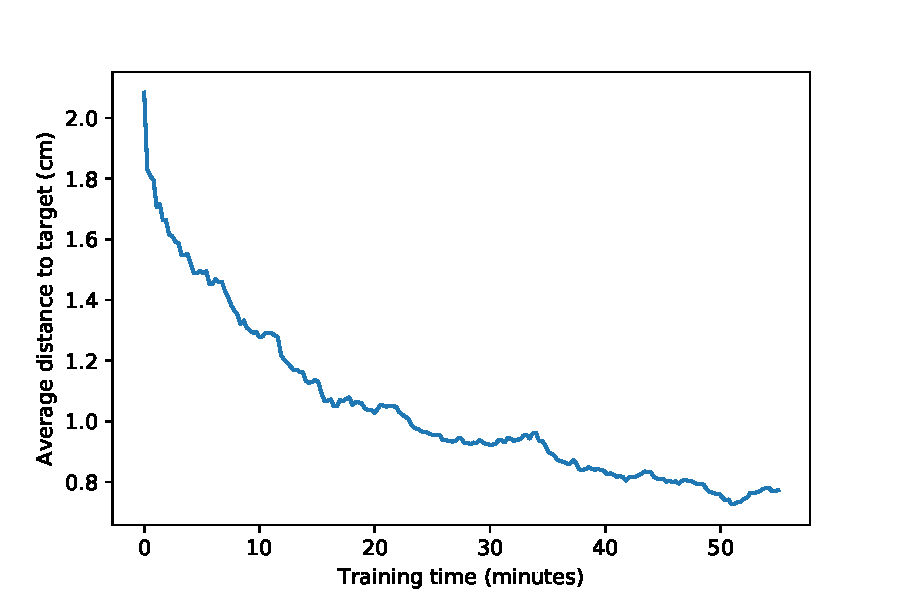
\includegraphics[width=0.50 \textwidth]{res/uarm_moving_goal_progress.pdf}

    \caption{Average final distance to target pose.}
    \label{fig:uarm_moving_goal_progress}
    
\end{figure}

\begin{figure}[h]
    \centering
    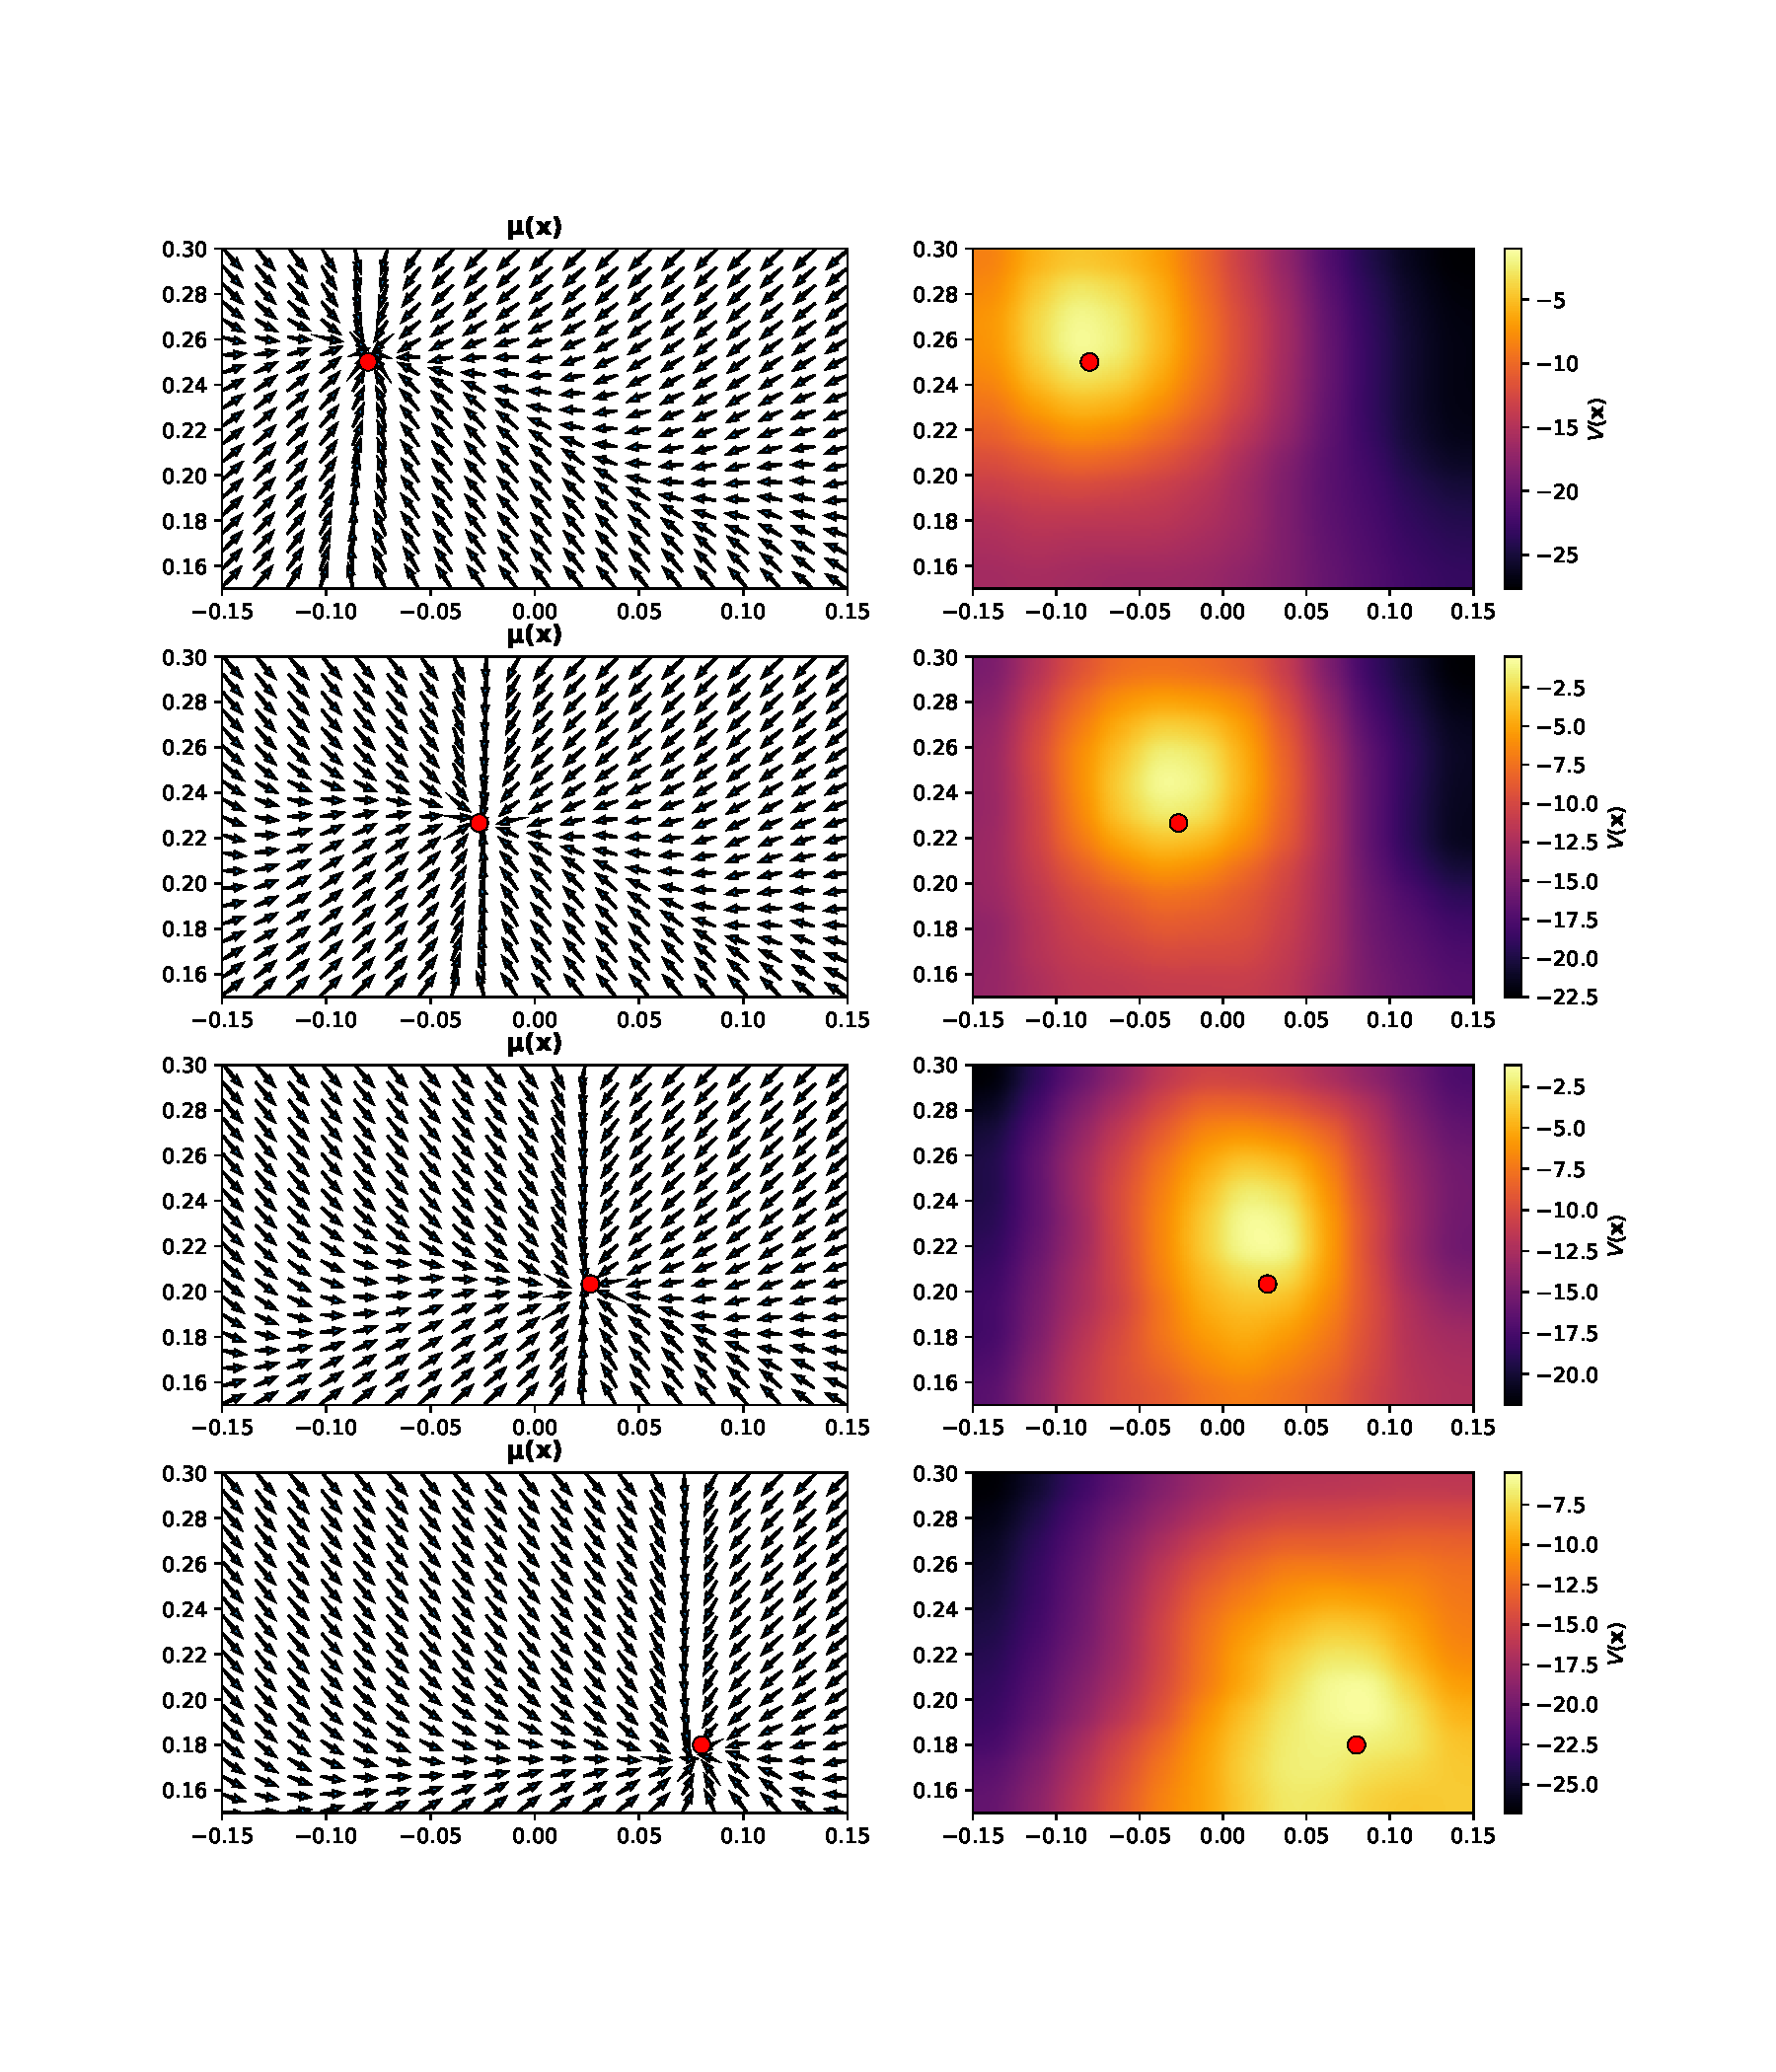
\includegraphics[width=\textwidth]{res/multiple_goals_uarm.pdf}

    \caption{Robot multiple goal poses of EEF}
    \label{fig:uarm_moving_goal_policy}
    
\end{figure}

%\begin{figure}[h]
%    \centering
%    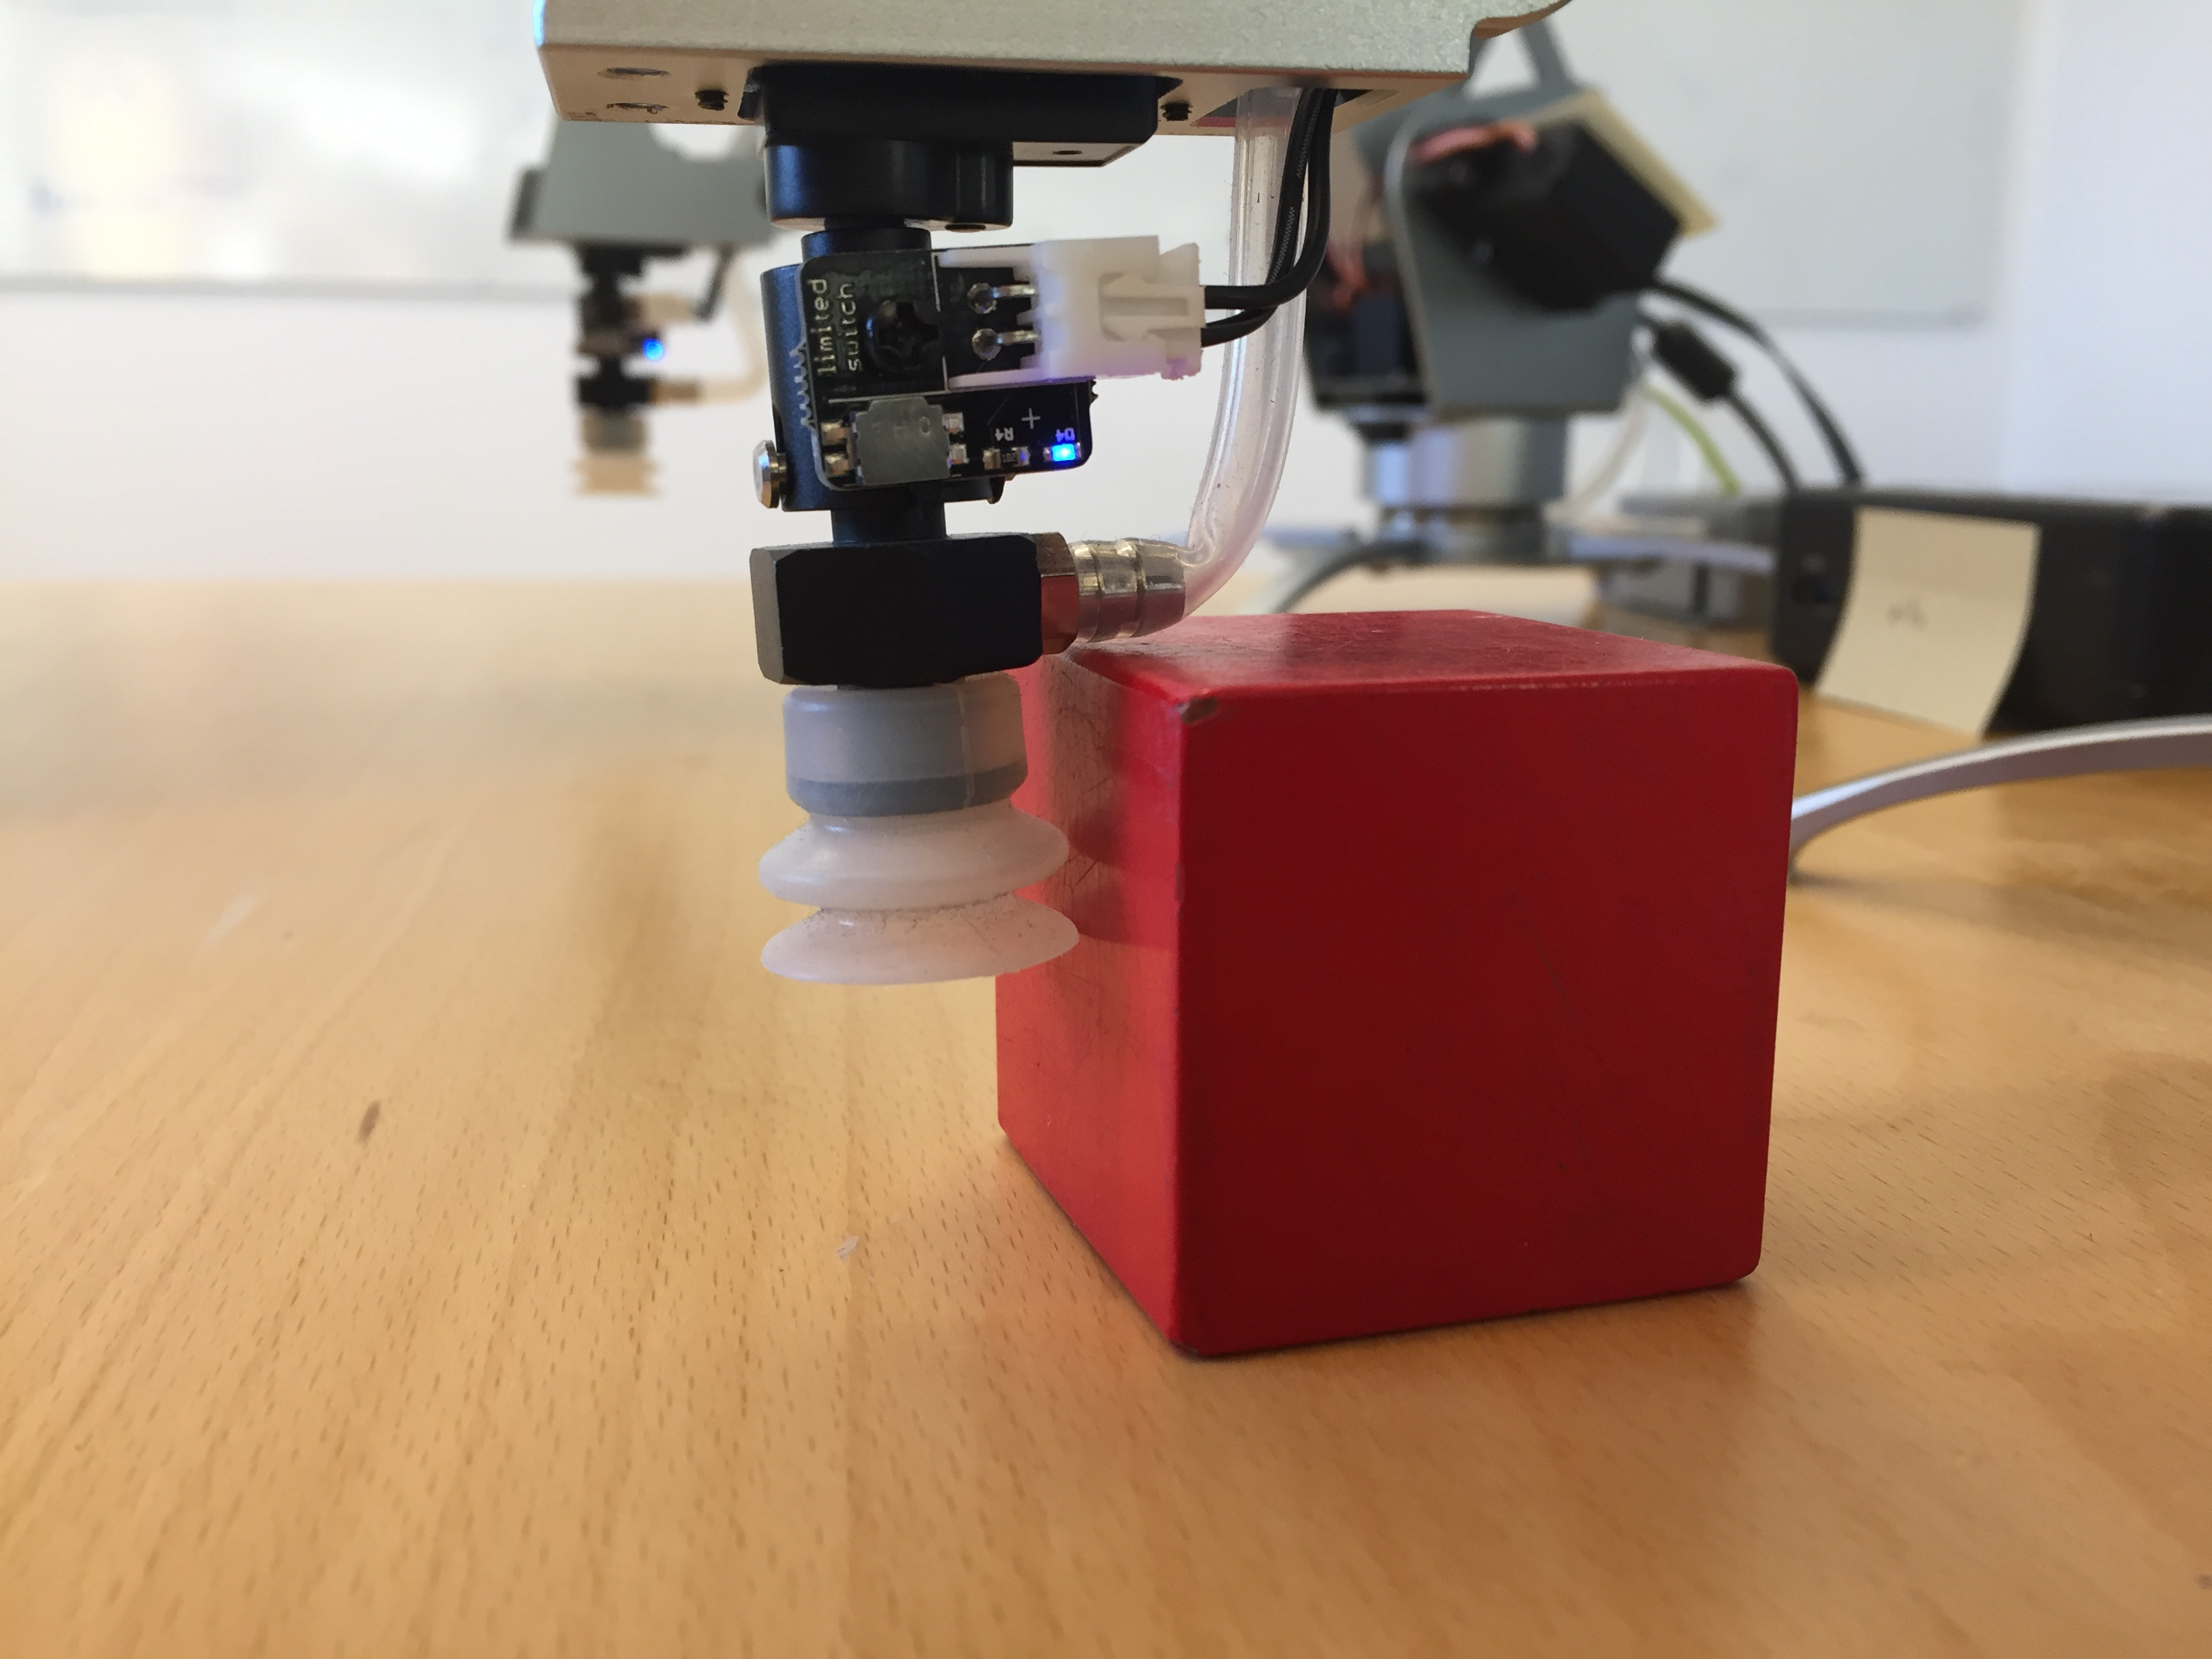
\includegraphics[width=0.40 \textwidth]{res/eef_cube_low.jpg}
%    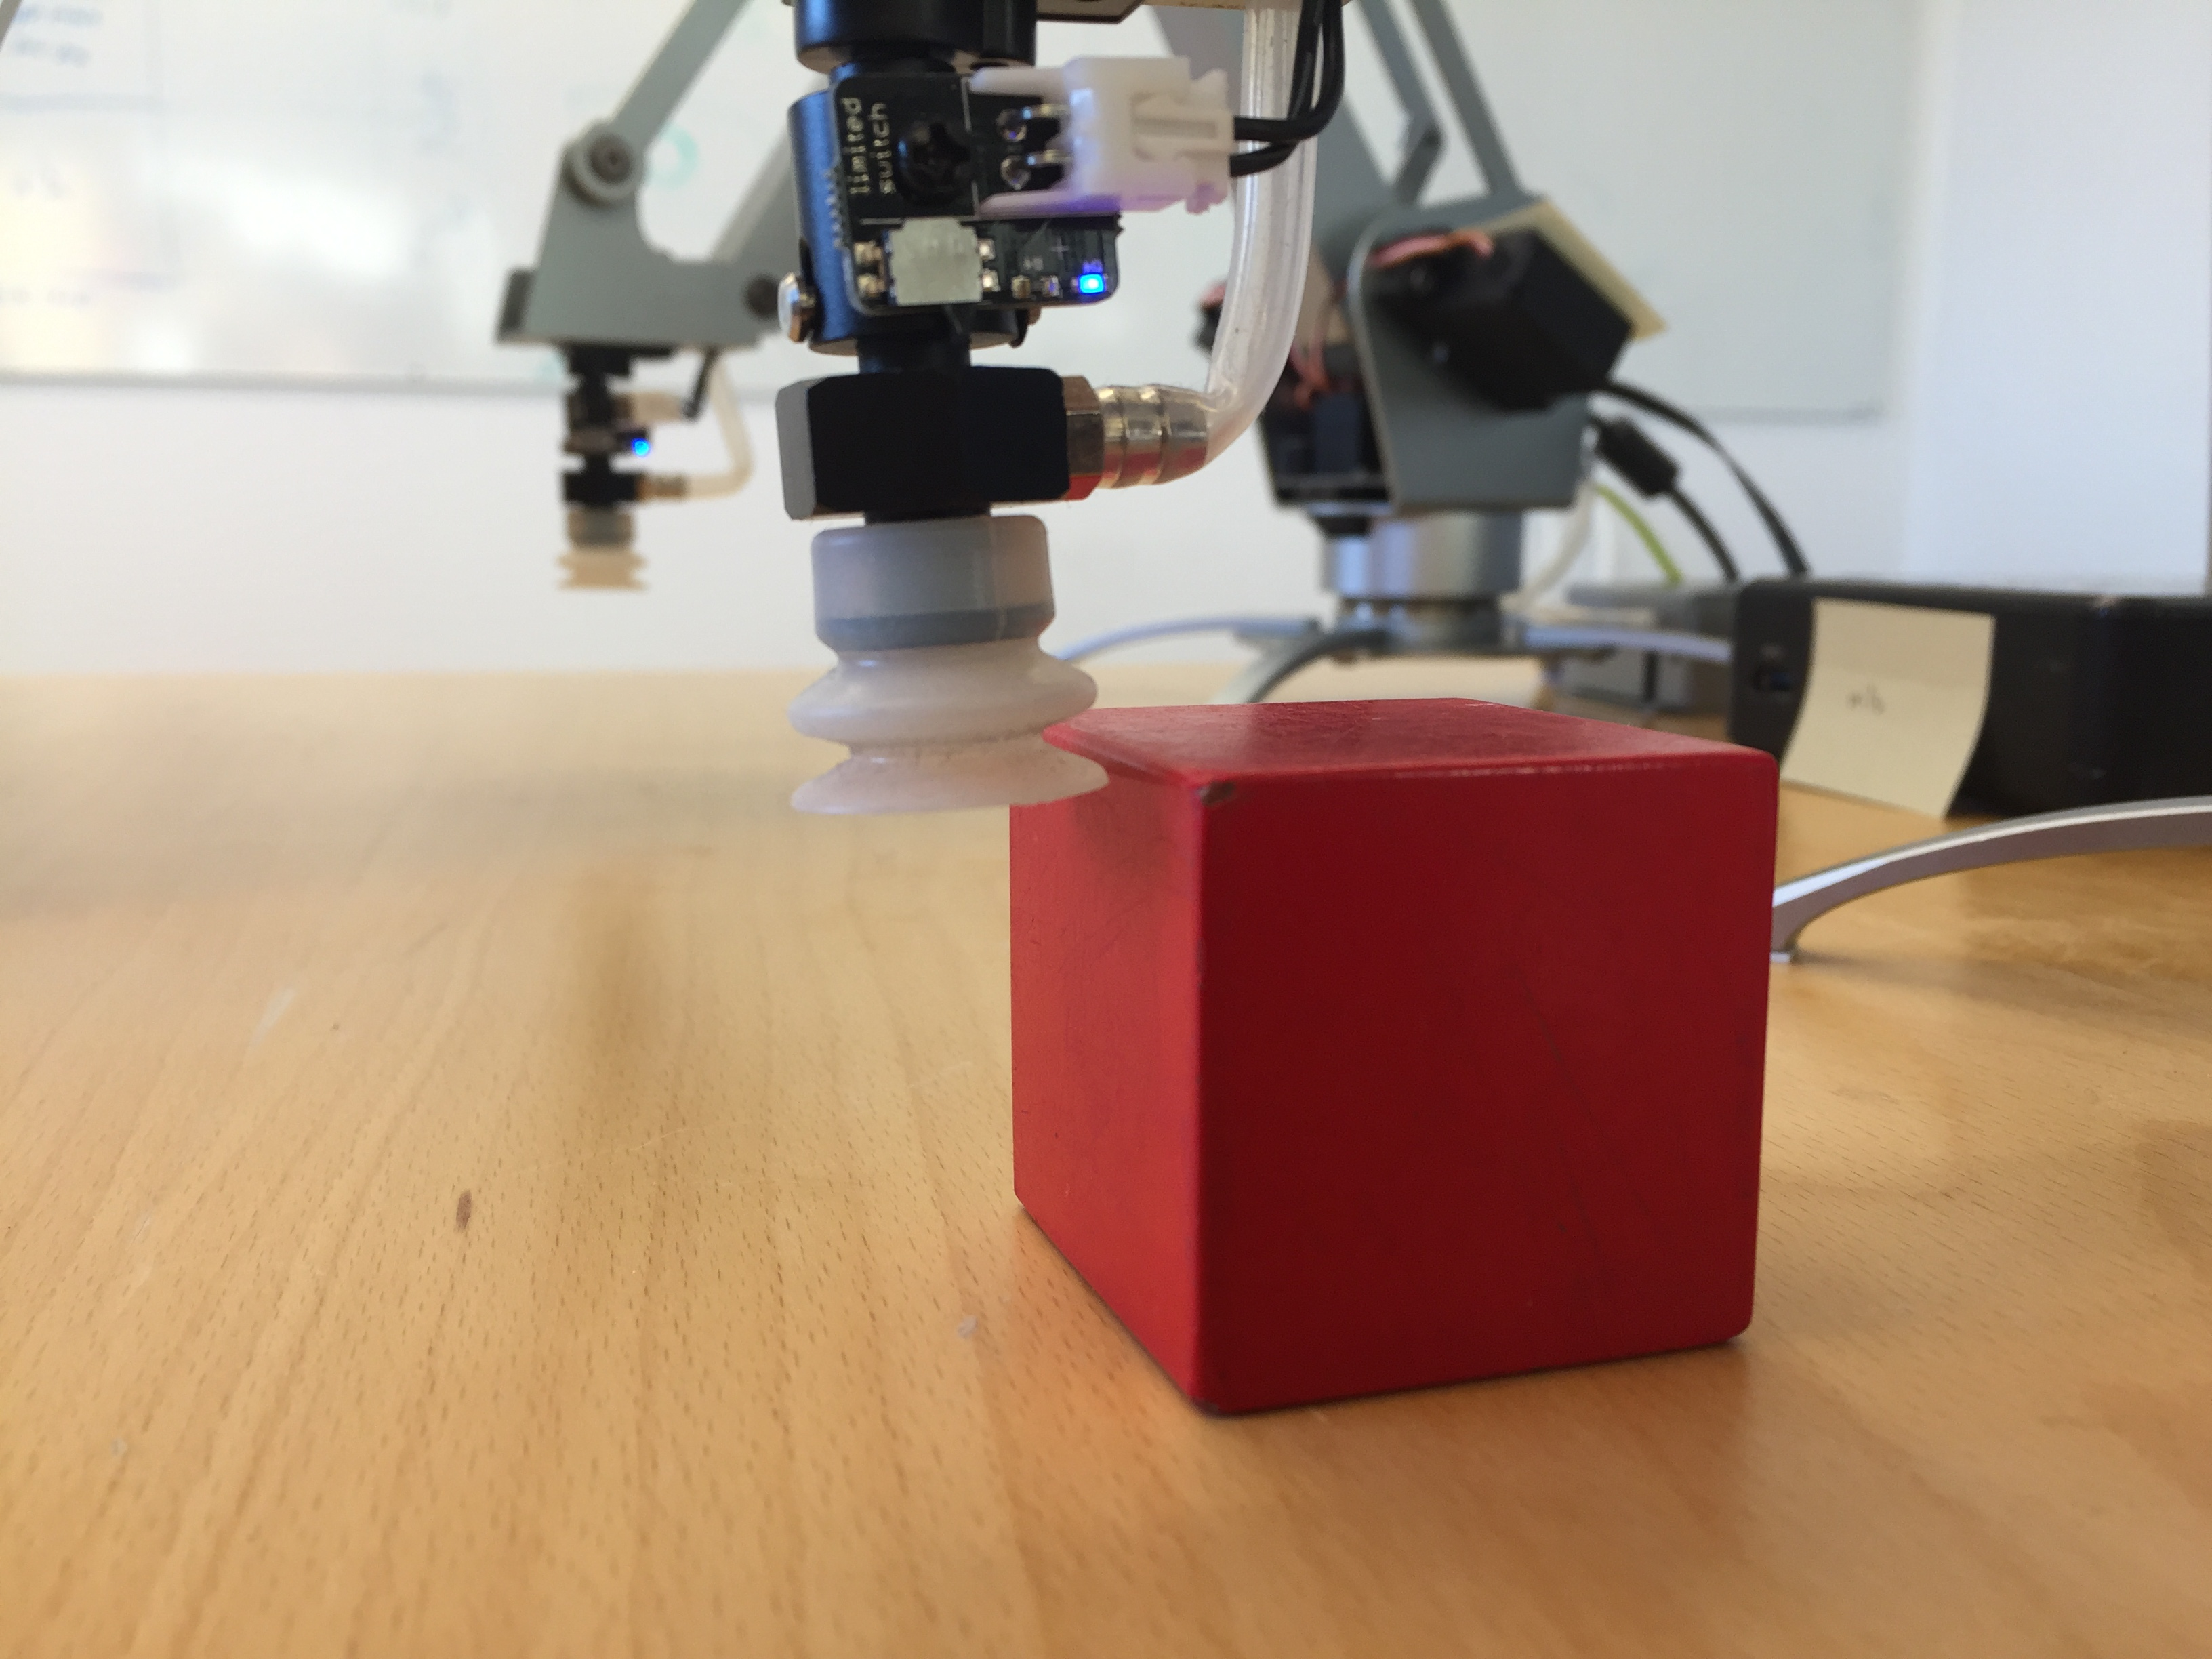
\includegraphics[width=0.40 \textwidth]{res/eef_cube_high.jpg}
%
%    \caption{Possible $z$-values of the eef. TODO: Finish/polish this}
%    
%\end{figure}
